\documentclass[11pt]{scrartcl}
\usepackage[boxthm,noasy]{evan}
\renewcommand{\S}{\ensuremath{\mathsection}}
\renewcommand{\labelitemi}{\ensuremath{\bullet}}
\usepackage{tikz}

\title{Week 1 Problem Set: Contradiction and Induction}
\author{Claude}
\date{Due Sunday 22 November 2026, 11:59 pm}

\begin{document}
\maketitle

\section*{Required problems (10 points each)}

\begin{problem}[P\&B 1]
  Prove that $\sqrt2 + \sqrt3 + \sqrt5$ is an irrational number.
\end{problem}

\begin{problem}[P\&B 2]
  Show that no set of nine consecutive integers can be partitioned into two sets with the product
  of the elements of the first set equal to the product of the elements of the second set.
\end{problem}

\begin{problem}[P\&B 3]
  Find the least positive integer $n$ such that any set of $n$ pairwise relatively prime integers
  greater than $1$ and less than $2005$ contains at least one prime number.
\end{problem}

\begin{problem}[P\&B 6]
  Show that there does not exist a function $f \colon \ZZ \to \{1, 2, 3\}$ satisfying
  $f(x) \neq f(y)$ for all $x, y \in \ZZ$ such that $\abs{x - y} \in \{2, 3, 5\}$.
\end{problem}

\begin{problem}[P\&B 7]
  Show that there does not exist a strictly increasing function $f \colon \NN \to \NN$ satisfying
  $f(2) = 3$ and $f(mn) = f(m) f(n)$ for all $m, n \in \NN$.
\end{problem}

\begin{problem}[P\&B 14]
  Prove that $3^n \geq n^3$ for all positive integers $n$.
\end{problem}

\begin{problem}[P\&B 16]
  Let $n$ be a positive integer. Prove that
  \[
    1 + \frac{1}{2^3} + \frac{1}{3^3} + \dots + \frac{1}{n^3} < \frac32.
  \]
\end{problem}

\begin{problem}[P\&B 18]
  Prove that for any $n \geq 1$, a $2^n \times 2^n$ checkerboard with a $1 \times 1$ corner square
  removed can be tiled by L-shaped pieces made of three unit squares:
  \begin{center}
  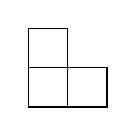
\begin{tikzpicture}[scale=0.5]
    \draw (0,0) rectangle (1,1); \draw (1,0) rectangle (2,1); \draw (0,1) rectangle (1,2);
  \end{tikzpicture}
  \end{center}
\end{problem}

\section*{Challenge problems (bonus)}

\begin{problem}[P\&B 9]
  Show that the interval $[0, 1]$ cannot be partitioned into two disjoint sets $A$ and $B$
  such that $B = A + a$ for some real number $a$.
\end{problem}

\begin{problem}[P\&B 19]
  Given a sequence of integers $x_1, x_2, \dots, x_n$ whose sum is $1$, prove that exactly one of
  the cyclic shifts
  \[
    x_1, x_2, \dots, x_n; \quad x_2, \dots, x_n, x_1; \quad \dots; \quad x_n, x_1, \dots, x_{n-1}
  \]
  has all of its partial sums positive. (A partial sum is the sum of the first $k$ terms, $k \leq n$.)
\end{problem}

\end{document}
